
\documentclass[12pt,letterpaper]{article}

% Packagess
\usepackage[utf8]{inputenc}
\usepackage{amsmath}
\usepackage{amssymb}
\usepackage{graphicx}
\usepackage{float}
\usepackage{geometry}
\usepackage{hyperref}
\usepackage{pdfpages}

% Page margins
\geometry{margin=1in}

% Document information
%\title{PHYS 2801 - Assignment}
%\author{Son Thanh Truong}
%\date{\today}


\begin{document}

\begin{titlepage}
    \centering
    \vspace*{3cm}

    {\Huge\bfseries Refractive Index of a Prism\par}

    \vspace{2cm}

    {\Large Son Thanh Truong\par}
    {\Large Student ID: 100972716\par}
    \vspace{0.5cm}
    {\large Carleton University\par}
    {\large PHYS 2007\par}
    {\large Lab Section: C\par}
    {\large Lab Partner: Lauren Gilchrist\par}
    {\large Date of Report Submission: \today\par}
    
    
    \vfill

    {\large \today\par}
\end{titlepage}


%\begin{document}

%\maketitle

\section{Question 1}

Describe the apparatus used in this experiment. Provide a ray diagram of the
spectrometer setup when light is refracted at minimum deviation in the prism.

Answer: The apparatus composes of a protractor grid surrounding a lens holder in the middle
with two telescopes, one faced the lamp to receive light through an adjustable slit.
The other telescope guides the light towards the eyes of the observer.

\section{Question 2}

Identify four to six discrete lines visible in the mercury spectrum. Report an error on
the angle measurement. Record the angle position of the turning points for all the
identified spectral lines, describe their relative intensity, and present your data in a
table.

AnswerThe error on the measurement is half a minute

\section{Question 3}



\section{Question 4}




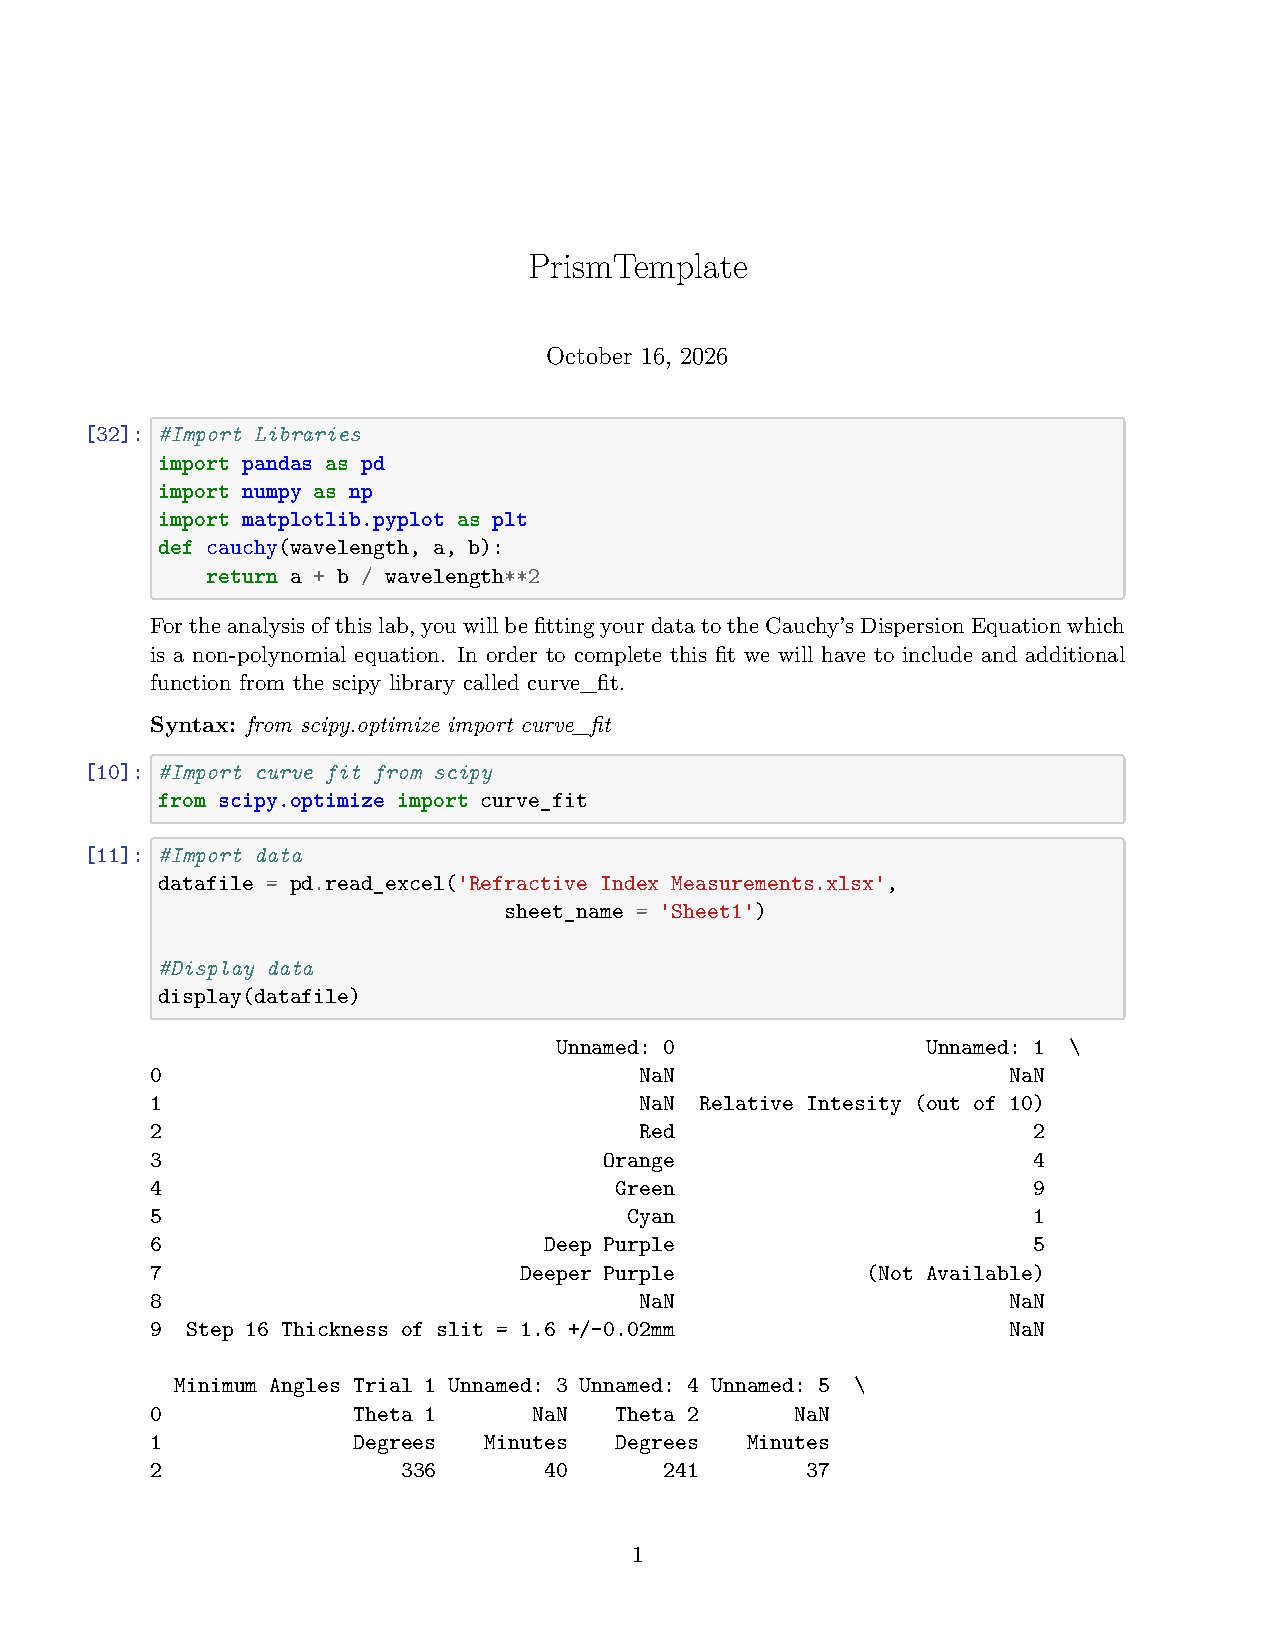
\includepdf[pages=-]{PrismTemplate.pdf}

\end{document}
